\documentclass{article}
\usepackage{parskip}
\usepackage{graphicx}
\usepackage{hyperref} % must be last import

\newcommand{\projectname}{Decentraliseret dataudveksling i notesapplikation}
\newcommand{\student}{Marcus Haukelid Larsen}
\newcommand{\supervisor}{?}

\begin{document}

\pdfbookmark[1]{Forside}{frontpage}

\begin{center}
  {\Huge \textbf{\projectname}}

  \vspace*{\fill}

  {\Large \textbf{\student}}

  \vspace*{\fill}

  {\large \textbf{Procesrapport}}
\end{center}

\thispagestyle{empty}

\newpage
\begin{center}  
  {\large \textbf{Elev:} \student}
  \vspace*{\fill}

  {\large \textbf{Projektnavn:} \projectname}
  \vspace*{\fill}

  {\large \textbf{Uddannelsessted:} Techcollege, Struervej 70, 9220 Aalborg Øst, Denmark}
  \vspace*{\fill}

  {\large \textbf{Elevplads:} RTX A/S , Strømmen 6, 9400 Nørresundby, Denmark}
  \vspace*{\fill}

  {\large \textbf{Projektperiode:} 05/02-2026 - 17/03-2026}
  \vspace*{\fill}

  {\large \textbf{Afleveringsdato:} 17/03-2026}
  \vspace*{\fill}

  {\large \textbf{Fremlæggelsesdato:} 20 el. 23/03-2026}
  \vspace*{\fill}

  {\large \textbf{Vejleder:} \supervisor}
  \vspace*{\fill}

  {\large \textbf{Underskrift:}}
  \vspace*{\fill}
  
  \begin{tabular}{p{6cm} p{6cm}}
    \hrulefill & \hrulefill \\
    Vejleder (\supervisor) & Elev (\student)
  \end{tabular}
\end{center}

\thispagestyle{empty}

\newpage
\tableofcontents

\newpage

\section{Læsevejledning}
Denne rapport er struktureret, så læseren først får en introduktion til
projektets kontekst. I indledningen præsenteres baggrunden for casen
og de centrale spørgsmål, som rapporten søger at besvare.

Efter indledningen følger en beskrivelse af projektplanlægningen, hvor
arbejdsprocessen og tidsplanen præsenteres.
Metodologiafsnittet forklarer, hvordan projektet er gennemført, og er
opdelt i tre underafsnit: Brugergrænseflade, Databehandling og Datalagring.

Rapporten afsluttes med en diskussion af projektets begrænsninger samt en
konklusion, som opsummerer de væsentligste resultater og erfaringer.

\section{Indledning}
Vi lever i en digitaliseret verden, hvor ejerskab i stigende grad erstattes af
midlertidig adgang.

Som følge af magtkoncentration er der opstået flere organiserede bevægelser, der
fremhæver decentraliseret digital infrastruktur som et muligt alternativ.

Decentralisering rejser nye politiske spørgsmål om ansvar, regulering og ulighed.
Fraværet af centrale aktører kan vanskeliggøre både kontrol og retlig beskyttelse.

Rapporten beskriver, hvordan produktet er udarbejdet, hvilke delelementer det
indebærer, og hvilke begrænsninger der er identificeret undervejs.

\section{Casebeskrivelse}
Vi lever i en digitaliseret verden, hvor ejerskab i stigende grad
erstattes af midlertidig adgang. Denne udvikling rejser politiske
spørgsmål om magt, rettigheder og afhængighed i relationen mellem
borgere, stater og globale tech-giganter. Når data fungerer som den
centrale valuta i den digitale økonomi, forskydes magten fra borgeren
til de platforme, der kontrollerer indsamling, behandling og
anvendelse af disse data.

Som reaktion på denne magtkoncentration er der opstået flere
organiserede bevægelser, som fremhæver decentraliseret digital
infrastruktur som et muligt alternativ. I en decentraliseret model
er data og digitale aktiver ikke samlet hos enkelte platforme, men
distribueret på tværs af netværk, hvor brugerne i højere grad 
har kontrol over egne oplysninger og digitale ressourcer.

Decentralisering rejser dog også nye politiske spørgsmål om ansvar,
regulering og ulighed. Fraværet af centrale aktører kan vanskeliggøre
både demokratisk kontrol og retlig beskyttelse, hvilket udfordrer
statens traditionelle rolle som garant for borgernes rettigheder.

\section{Problemformulering}
Hvordan kan decentraliseret dataudveksling i en notesapplikation
bidrage til øget digitalt ejerskab og reducere brugerens afhængighed af
centrale platforme uden at gå på kompromis med tilgængelighed og 
brugervenlighed?

\section{Projektplanlægning}
\begin{figure}[h]
  \centering
  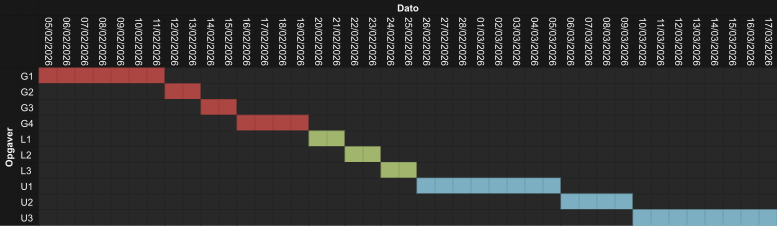
\includegraphics[width=1\textwidth]{tidsplan.png}
  \caption{Gantt-diagram}
\end{figure}

\section{Metodologi}
\subsection{Brugergrænseflade}
\subsection{Databehandling}
\subsection{Datalagring}

\section{Begrænsninger}

\section{Konklusion}

\end{document}
